\documentclass{article}
\usepackage{amsmath}
\usepackage{enumitem}
\usepackage{graphicx}
\title{Project Report — Ice-Ocean Interaction}
\author{David Sermoneta, Emma Bastås}

\begin{document}
\maketitle

\subsection*{Numerical Methods used}

\noindent For the discretization, we used a uniform scheme with a total of 1000 discretization points. This is the case for all the plots created in this project.

\subsubsection*{Interpolation of velocity-data}

We used cubic spline to interpolate the velocity-data. Later on we'll want to compute the derivative (see next section) of this interpolation and thus linear interpolation is ruled out as an alternative as it isn't differentiable at all points. That leaves us with cubic spline and Lagrange interpolation to choose from. Generally Lagrange interpolation \emph{can} suffer from Runge's phenomenon, but in our case this wouldn't be a problem. We conclude there isn't a good reason to pick one of cubic spline and Lagrange over the other for our specific case.

\begin{itemize}
    \item[] \textbf{Pro:} Easy to work with when differentiating as it is $C^1$ continuous
    \item[] \textbf{Con:} If the input is bad, even by a little bit, any non-linear interpolation method is very sensitive and can give rise to high errors. This is due to the high condition number associated with these types of functions.
\end{itemize}

\subsubsection*{Derivative of velocity-data}
We have velocity data (Table 1 in the assignment PDF), and interpolated it in the previous section. But equation (1) in the assignment PDF uses the derivative of the velocity (after expanding with the product rule) with regards to $x$ (distance from plume). We use a forward difference scheme to approximate the derivative, it's implemented in \texttt{approximate\_derivative}.

\begin{itemize}
    \item[] \textbf{Pro:} Extremely easy to implement and to understand.
    \item[] \textbf{Con:} The error is $\mathcal{O}(h)$, unlike central difference which has $\mathcal{O}(h^2)$
\end{itemize}

\subsubsection*{Solving of the temperature and salinity BVP-ODE}

The temperature and salinity are both given by equation (1) in the assignment PDF, the boundary conditions are the only things that differ. As such we use same methods for both, described below.

\noindent We used finite difference method for this BVP-ODE, with centered difference to approximate the temperature/salinity derivatives. Our scheme is implemented in \texttt{solve\_ODE}.

\begin{itemize}
    \item[] \textbf{Pro:} Centered difference is explicit, making it easier to implement than backwards-Euler. This is simultaneously a con since convergence isn't guaranteed for explicit methods.
    \item[] \textbf{Con:} The number of discretization points for the finite difference method is limited by computer memory as each equation for each discretization point has to be stored in memory at the same time. On our machine we ran into problems at $N \approx 100,000$. An iterative method on the other hand doesn't suffer from this problem to the same degree, as it iteratively updates a smaller matrix, consuming less memory.
\end{itemize}

\subsubsection*{Approximation of density}

As described by Asay-Davis et al\footnote{Asay-Davis, X. S., Cornford, S. L., Durand, G., Galton-Fenzi, B. K., Gladstone, R. M., Gudmundsson, G. H., Hattermann, T., Holland, D. M., Holland, D., Holland, P. R., Martin, D. F., Mathiot, P., Pattyn, F., and Seroussi, H.: Experimental design for three interrelated marine ice sheet and ocean model intercomparison projects: MISMIP v. 3 (MISMIP +), ISOMIP v. 2 (ISOMIP +) and MISOMIP v. 1 (MISOMIP1), Geosci. Model Dev., 9, 2471–2497, https://doi.org/10.5194/gmd-9-2471-2016, 2016. } the density can be approximated as a function of temperature and salinity. We've used this same formula, implemented in \texttt{density\_approximation}.


\subsubsection*{Notes on other built-in functions}

We use \texttt{numpy.linalg.solve} to solve the equation given by our finite difference scheme. This function is highly optimized (uses LAPACK under the hood) for solving linear equations of this kind. It uses LU-decomposition with partial pivoting.

\begin{figure}[t]
    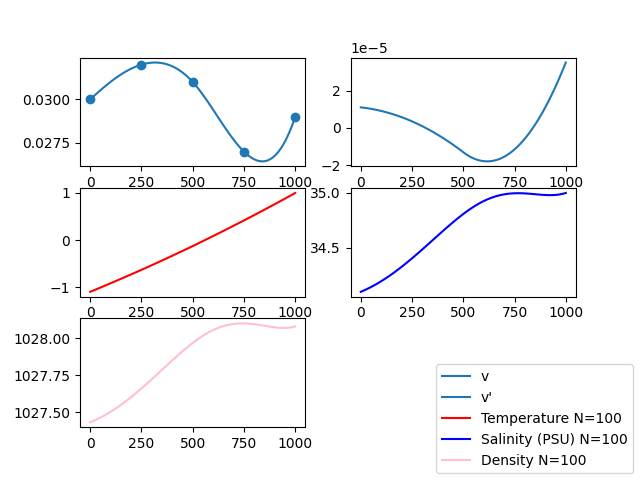
\includegraphics{Plots.png}
    \caption{Plots}
\end{figure}

\end{document}
